\section{Introduction}

\begin{frame}{Probing the EW Sector and BSM Physics with $W^\pm Zjj$}
    \begin{itemize}
        \setlength{\itemsep}{1.5em} % Spazio per riempire bene la slide senza affollarla
        
        \item \textbf{Dataset:} $140\,\unit{fb}^{-1}$ of $pp$ collisions at $\sqrt{s} = 13\,\unit{TeV}$ (2015--2018).
        
        \item \textbf{Target:} Fully leptonic decays of $W^\pm Zjj$ production.
        
        \item \textbf{Measurements:} Integrated \& differential fiducial cross-sections ($\sigma_{\text{EW}}$ and $\sigma_{\text{strong}}$).
        
        \item \textbf{Goal:} Isolate Vector Boson Scattering (VBS).
        
        \item \textbf{New Physics:} EFT limits on Anomalous Quartic Gauge Couplings (aQGC).
    \end{itemize}
\end{frame}

% =======================================================================

\begin{frame}{The ATLAS Detector}
    \begin{center}
                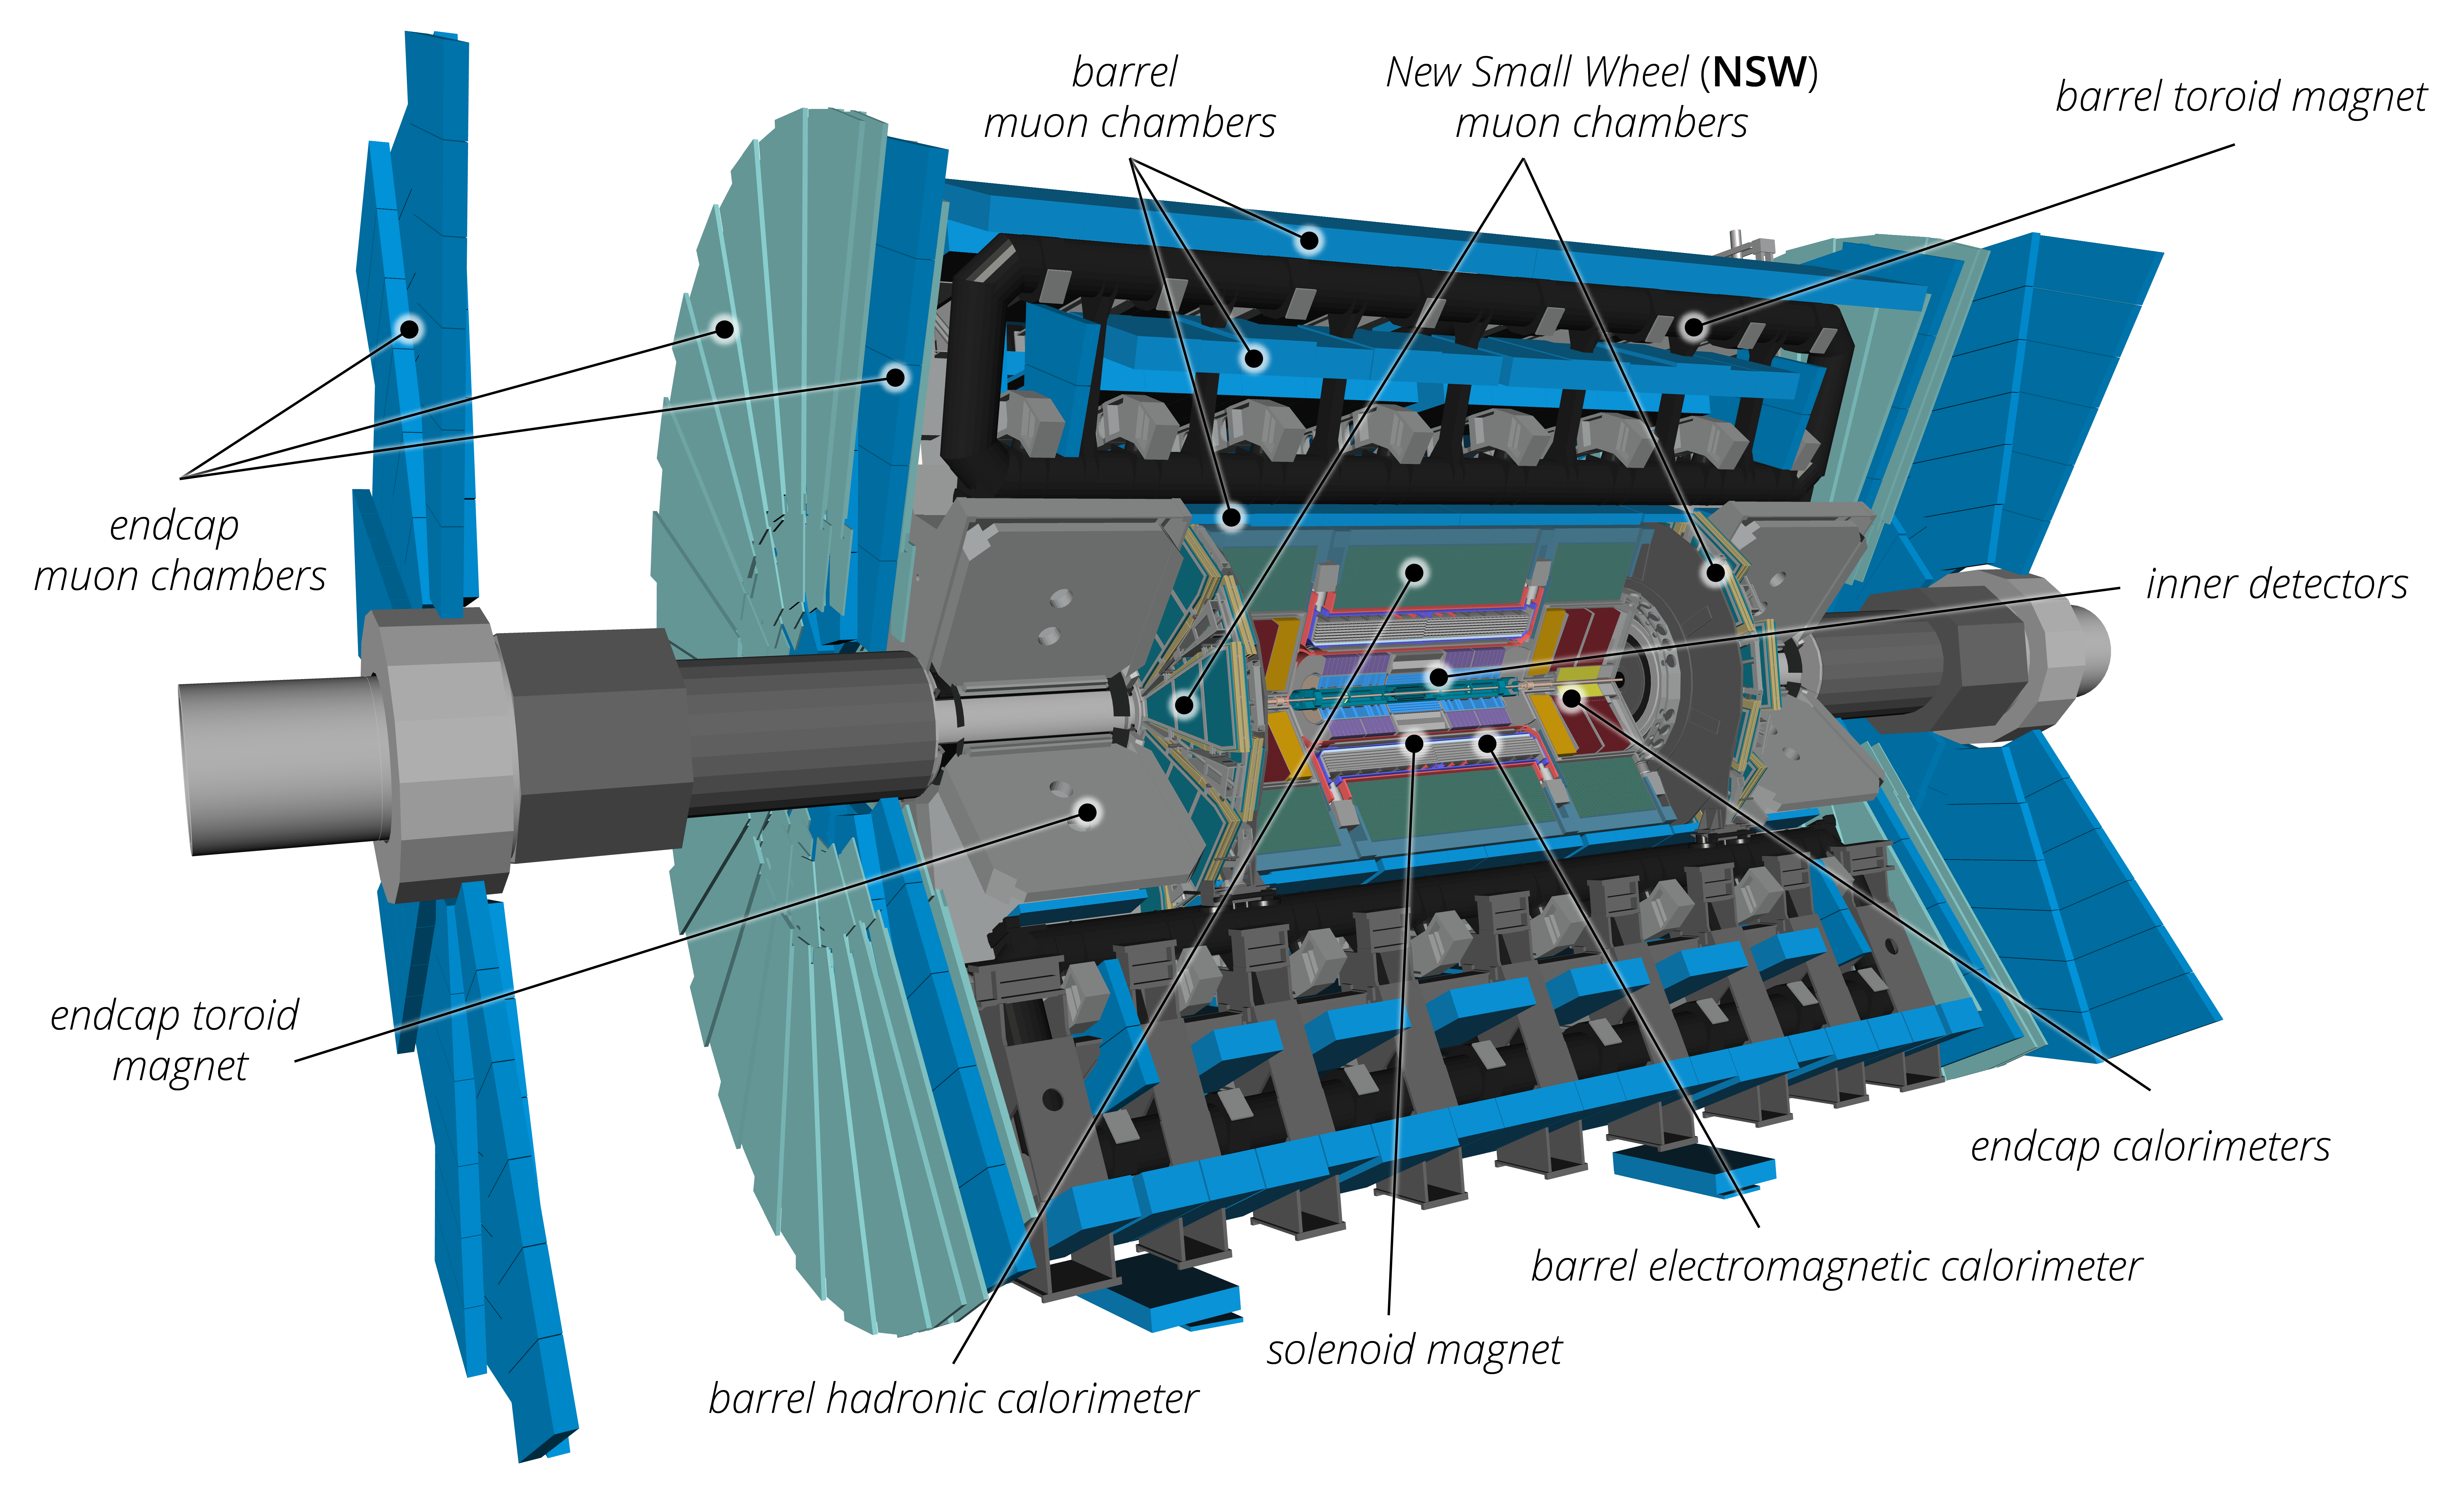
\includegraphics[width=0.8\textwidth]{assets/fig_02.png}
            \end{center}
\end{frame}

\section{Theoretical Framework}
\begin{frame}{Gauge Boson Self-Interactions}
    \begin{itemize}
        \item The Electroweak (EW) sector of the Standard Model is based on the \textbf{non-abelian} gauge symmetry $SU(2)_L \times U(1)_Y$.
        \item Unlike QED, the generators of $SU(2)_L$ do not commute. As a consequence, the physical vector bosons ($W^\pm, Z, \gamma$) self-interact.
        \item This structure directly dictates the existence of \textbf{Triple} (TGC) and \textbf{Quartic} (QGC) Gauge Couplings:
    \end{itemize}
    
    \begin{equation*}
        \mathcal{L}_{\text{TGC}} = \frac{1}{2}g \epsilon_{abc} W_b^\mu W_c^\nu (\partial_\mu W_{a\nu} - \partial_\nu W_{a\mu}) \qquad  \mathcal{L}_{\text{QGC}}= \frac{1}{4}g^2 \epsilon_{abc} \epsilon_{ars} W_b^\mu W_c^\nu W_{r\mu} W_{s\nu} 
    \end{equation*}
 Probe these vertices to test the SM rigidity and search for anomalous couplings (aQGC) arising from New Physics.
\end{frame}

\begin{frame}{Experimental Signature: Vector Boson Scattering}
    \textbf{Vector Boson Scattering} (VBS) $VV\to VV$ with $V=W/Z/\gamma$, is a key process with which to probe the $SU(2)_L\times U(1)_Y$ gauge symmetry of the \textbf{electroweak} (EW) theory that determines the \textbf{self-couplings} of vector bosons. To study these couplings, we exploit the purely electroweak production of \textbf{$W^\pm Zjj$}. 


    \begin{center}
    \begin{tikzpicture}
        \node[inner sep=0pt] (ew_figs) at (0,0) {
            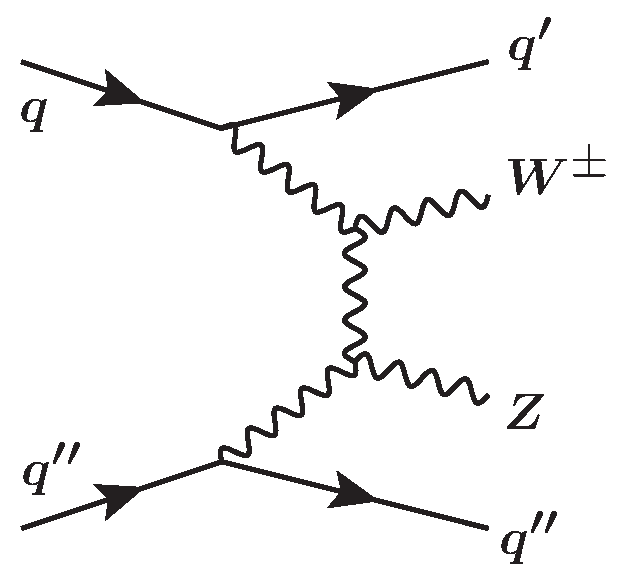
\includegraphics[width=0.18\textwidth]{Immagini/fig_01a.pdf}\hspace{0.2cm}
            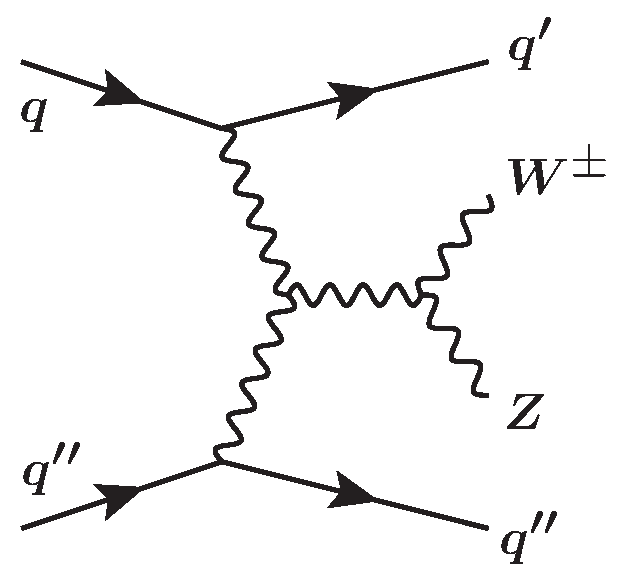
\includegraphics[width=0.18\textwidth]{Immagini/fig_01b.pdf}\hspace{0.2cm}
            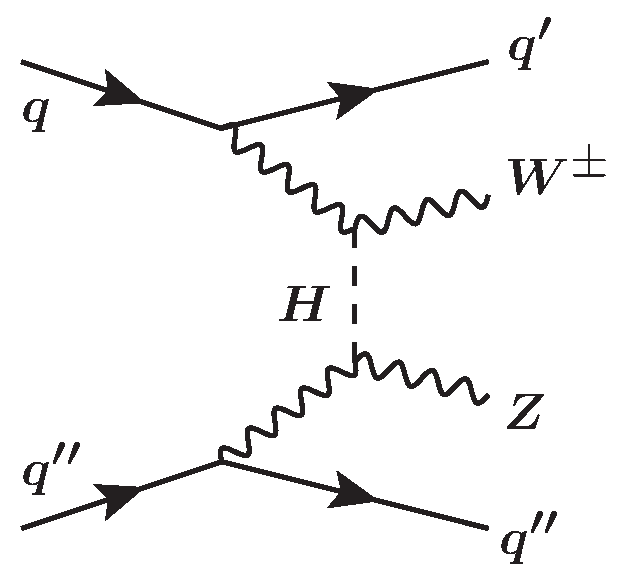
\includegraphics[width=0.18\textwidth]{Immagini/fig_01c.pdf}\hspace{0.2cm}
            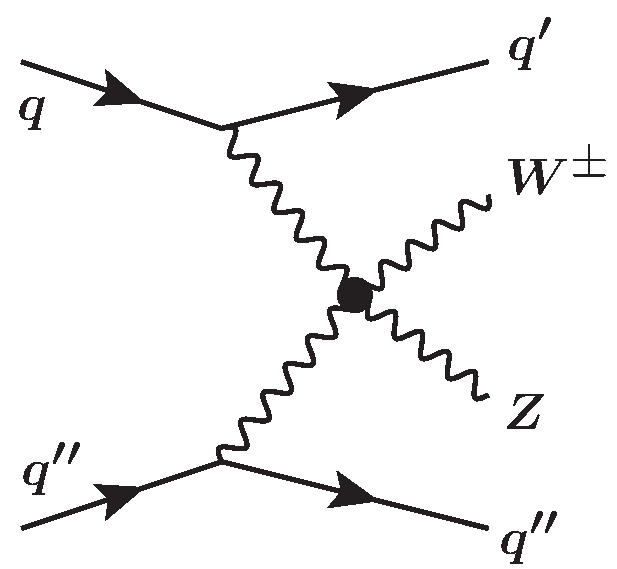
\includegraphics[width=0.18\textwidth]{Immagini/fig_01d.pdf}
        };
        \draw[red, thick, rounded corners=3pt] 
            ([xshift=-0.1cm, yshift=-0.1cm]ew_figs.south west) rectangle 
            ([xshift=0.1cm, yshift=0.1cm]ew_figs.north east);
        \node[red, right, font=\bfseries] at ([xshift=0.2cm]ew_figs.east) {$W^\pm Zjj$-EW};
        \node[inner sep=0pt] (qcd_figs) at (0,-2.5) {
            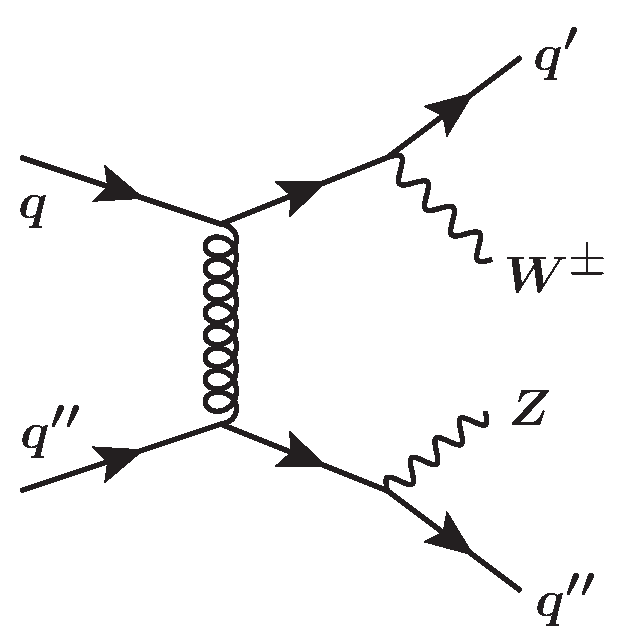
\includegraphics[width=0.16\textwidth]{Immagini/fig_02a.pdf}\hspace{0.2cm}
            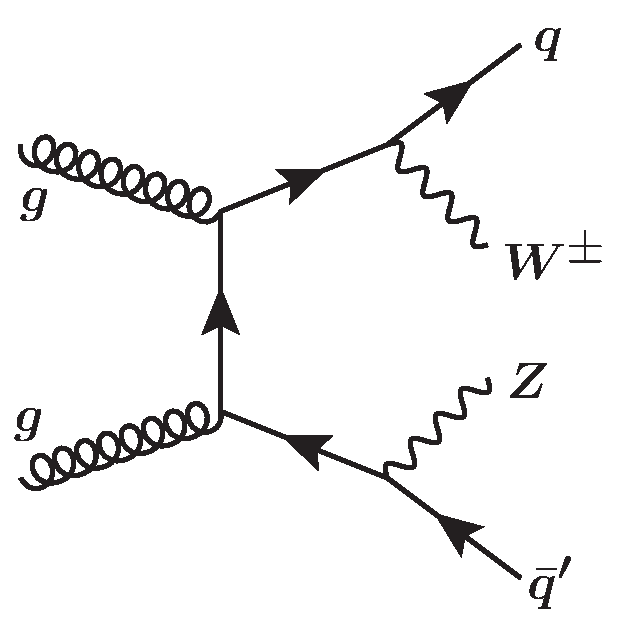
\includegraphics[width=0.16\textwidth]{Immagini/fig_02b.pdf}\hspace{0.2cm}
            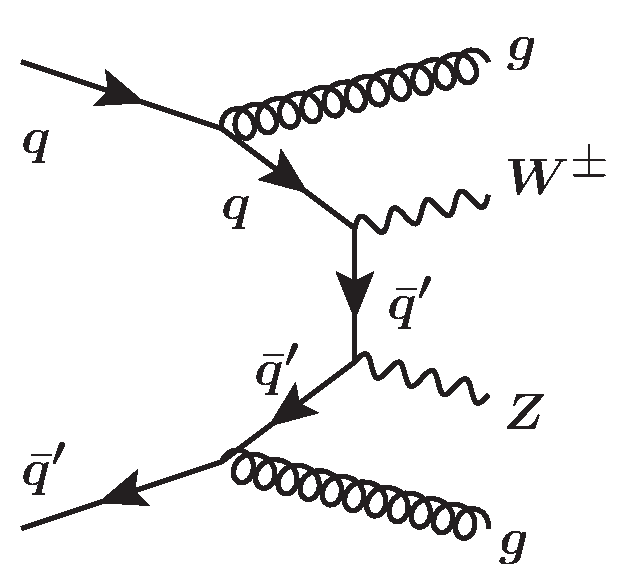
\includegraphics[width=0.16\textwidth]{Immagini/fig_02c.pdf}
        };
        \draw[blue, thick, rounded corners=3pt] 
            ([xshift=-0.1cm, yshift=-0.1cm]qcd_figs.south west) rectangle 
            ([xshift=0.1cm, yshift=0.1cm]qcd_figs.north east);
        \node[blue, right, font=\bfseries] at ([xshift=0.2cm]qcd_figs.east) {$W^\pm Zjj$-QCD};
        
    \end{tikzpicture}
    \end{center}
\end{frame}
\begin{frame}{A little look at the Effective Field Theory (EFT)}
    The $W^\pm Zjj$-EW production can be sensitive to effects beyond the SM affecting the quartic interactions of weak bosons. The measured $W^\pm Zjj$ events are therefore used to search for anomalous quartic gauge couplings (aQGC) using an EFT framework. In this model, the Lagrangian of the standard model is extended into an efficient Lagrangian by adding higher-order operators and their respective Wilson coefficients as follows:
    \begin{equation*}
        \mathcal{L}_{\mathrm{eff}} = \mathcal{L}_{\mathrm{SM}} + \sum_{i} \frac{f_{i}^{(6)}}{\Lambda^{2}} O_{i}^{(6)} + \sum_{j} \frac{f_{j}^{(8)}}{\Lambda^{4}} O_{j}^{(8)} + \dots 
    \end{equation*}
    Where:
    \begin{itemize}
        \item $O_{i,j}^{(6),(8)}$: are dimension-6 and dimension-8 operators;
        \item $f_{i}^{(6)}$ e $f_{j}^{(8)}$: dimensionless couplings
        \item $\Lambda$: is the energy scale of the new processes
    \end{itemize}
\end{frame}
\begin{frame}{A little look at the Effective Field Theory (EFT)}
    The squared scattering amplitude of the effective field theory predicion for $W^\pm Zjj$ production can be written as:
    \begin{equation*}
        \left| A_{\mathrm{SM}}+\sum_i c_i A_i \right|^2 = {\left| A_{\mathrm{SM}} \right| }^2 + \sum_i c_i \, 2 \mathrm{Re}(A^*_{\mathrm{SM}}A_i)+ \sum_i c_i^2 |A_i|^2 +\sum_{ij,i\neq j} c_i c_j \, 2 \mathrm{Re}(A_{i} A^*_{j})
    \end{equation*}
    \begin{itemize}
        \item $c_i = f_j^{(8)} / \Lambda^4$, $A_{\mathrm{SM}}$ is the SM scattering amplitude;
        \item $2 \operatorname{Re}(A^*_{\mathrm{SM}} A_i)$ is the amplitude of the interference term between the SM and the dimension-8 operators;
        \item $\sum_i {c_i}^2 |A_i|^2$ is the pure dimension-8 contribution, and $\sum_{ij,i\neq j} c_i c_j 2 \operatorname{Re}(A_i A^*_j)$ is the amplitude of interferences between two dimension-8 operators, called cross terms.
    \end{itemize}
\end{frame}

\section{Fiducial Phase Space and MC Simulations}

\begin{frame}{Fiducial Phase Space for Leptons}
    The $W^\pm Zjj$ cross-sections are measured in a fiducial phase space. Leptons produced in the decay of a hadron, a $\tau$-lepton, or their descendants are not considered in the definition of the fiducial phase space and are treated as background.
    
    \vspace{0.4cm} % Aggiunge un po' di respiro tra testo e tabella
    
    \begin{center}
    \small % Rimpicciolisce leggermente il font per far stare tutto comodamente
    \renewcommand{\arraystretch}{1.3} % Leggermente ridotto da 1.4 a 1.3 per ottimizzare lo spazio verticale
    \begin{tabular}{llc}
    \hline
    \textbf{Category} & \textbf{Kinematic Variable} & \textbf{Requirement} \\
    \hline
    $Z$ leptons & Transverse momentum ($p_T^{\ell_Z}$) & $> 15\,\text{GeV}$ \\
    $W$ lepton & Transverse momentum ($p_T^{\ell_W}$) & $> 20\,\text{GeV}$ \\
    All leptons & Pseudorapidity ($|\eta_\ell|$) & $< 2.5$ \\
    $Z$ boson & Invariant mass window ($|m_{\ell^+ \ell^-} - m_Z^{\text{PDG}}|$) & $< 10\,\text{GeV}$ \\
    $W$ boson & Transverse mass ($m_T^W$) & $> 30\,\text{GeV}$ \\
    Angular isolation & Distance between $Z$ leptons ($\Delta R(\ell_{Z1}, \ell_{Z2})$) & $> 0.2$ \\
    Angular isolation & Distance between $W$ and $Z$ leptons ($\Delta R(\ell_W, \ell_Z)$) & $> 0.3$ \\
    \hline
    \end{tabular}
    \end{center}
\end{frame}

\begin{frame}{Fiducial Phase Space for Jets}
    In addition, at least two jets are required, reconstructed using the anti-$k_t$ algorithm with radius parameter $R=0.4$. Hard processes with a $b$-quark in the initial or final states, such as $tZj$ production, are not considered as part of the $W^\pm Zjj$-EW events.
    
    \vspace{0.4cm} % Aggiunge un po' di respiro tra testo e tabella
    
    \begin{center}
    \small % Rimpicciolisce leggermente il font per far stare tutto comodamente
    \renewcommand{\arraystretch}{1.3} % Leggermente ridotto da 1.4 a 1.3 per ottimizzare lo spazio verticale
    \begin{tabular}{llc}
    \hline
    \textbf{Category} & \textbf{Kinematic Variable} & \textbf{Requirement} \\
    \hline
    All jets & Transverse momentum ($p_T^j$) & $> 40\,\text{GeV}$ \\
    All jets & Pseudorapidity ($|\eta_j|$) & $< 4.5$ \\
    Angular isolation & Distance between jets and leptons ($\Delta R(j, \ell)$) & $> 0.3$ \\
    Tagging jets & Opposite hemispheres ($\eta_{j1} \cdot \eta_{j2}$) & $< 0$ \\
    Tagging jets & Invariant mass ($m_{jj}$) & $> 500\,\text{GeV}$ \\
    \hline
    \multicolumn{3}{c}{\textbf{Jet Veto}} \\
    \hline
    $b$-quark jets & Absence of $b$-jets in initial/final state & $N_{b\text{-jet}} = 0$ \\
    \hline
    \end{tabular}
    \end{center}
\end{frame}

\begin{frame}{How to eliminate leptons ambiguity?}
    \begin{itemize}
        \item Leptons and final-state neutronos that do not originate from hadron or $\tau$-lepton decays, are matched to the $W^\pm$ and $Z$ boson decay products using an algorithmic approach, called the \textbf{resonant shape algorithm}. 
        \item This algorithm is based on the value of an estimator expressing the product of the nominal line-shapes of the $W$ and $Z$ resonances:
    \end{itemize}
   
    \vspace{0.4cm} % Aggiunge un po' di respiro tra testo e tabella

    \begin{equation*}
    P = \left| \frac{1}{ m^2_{(\ell^+,\ell^-)} - \left(m_Z^{\textrm{PDG}}\right)^2 + \textrm{i} \; \Gamma_Z^{\textrm{PDG}} \; m_Z^{\textrm{PDG}} } \right|^2  \times \; \left| \frac{1}{ m^2_{(\ell',\nu_{\ell'})} - \left(m_W^{\textrm{PDG}}\right)^2 + \textrm{i} \; \Gamma_W^{\textrm{PDG}} \; m_W^{\textrm{PDG}} } \right|^2 
\end{equation*}
\end{frame}

\begin{frame}{Monte Carlo Simulation of the Signal}
The simulation of $W^\pm Zjj$ events was primarily generated using the \texttt{MadGraph5\_aMC@NLO2.6.5} MC event generator, interfaced with \texttt{Pythia8.240}. The simulation was divided into distinct components:
\begin{itemize}
    \item \textbf{Electroweak production \wzjjew}: The actual signal. It is calculated at leading order (LO), considering purely electroweak processes (order $\alpha_\text{EW}^6$).
    \item \textbf{QCD production \wzjjqcd}: Considered a background for the VBS analysis. This component is calculated at next-to-leading order (NLO) in QCD.
    \item \textbf{Interference \wzjj-INT}: Quantifies the quantum interference between the EW and QCD production. It is calculated at LO and yields a positive contribution of 6\% in the fiducial region, reaching up to 12\% for events with three or more jets.
\end{itemize}
\end{frame}

\begin{frame}{Monte Carlo Simulation of the Background}
    In addition to the \wzjjqcd  \,production, there are numerous other Standard Model processes that can mimic the signal in the detector. These backgrounds fall into two categories based on how they are estimated:
    \begin{itemize}
    \item \textbf{Backgrounds with \textit{prompt} (real) leptons:} Processes such as the production of $ZZ$ pairs, $WW$, tribosons ($VVV$), or top quarks associated with vector bosons ($t\bar{t}V$, $tZj$). Their contribution is evaluated entirely using Monte Carlo simulations.
    \item \textbf{Backgrounds with \textit{fake} leptons:} Events where a hadronic jet is misidentified as a lepton by the detector. Being an instrumental artifact that is complex to simulate accurately, this background is estimated directly using data-driven techniques.
\end{itemize}
\end{frame}

\begin{frame}{Detector Simulation}
    All generated MC events were passed throught the ATLAS detector simulation, based om \texttt{Geant4}, and processed using the same recostruction software used for the data.

    Furthermore, the lepton and jet momentum scale and resolution, the lepton reconstruction, identification, isolation and trigger efficiencies and the pile-up jets and b-jet veto efficiencies in the simulation were corrected to match those measured in data.
\end{frame}
    
\section{Event selection \& Background estimation}
\begin{frame}{Event Selection: Physics Objects Definition}
    \textbf{Data Quality \& Trigger:}
    \begin{itemize}
        \item Only data with stable beams and fully operational sub-detectors.
        \item Single-lepton triggers used (Combined efficiency $\approx 99\%$ for offline-selected $W^\pm Zjj$ events).
    \end{itemize}
    \vspace{0.3cm}
    \textbf{Physics Objects Reconstruction:}
    \begin{itemize}
        \item \textbf{Prompt Leptons} $e, \mu, \nu$ $(E_T^{miss})$: Reconstructed combining ID tracks with ECAL clusters or MS tracks. Strict isolation and impact parameter criteria are applied to reject non-prompt background.
        \item \textbf{Hadronic Jets:} Clustered using the \textit{anti-$k_t$} algorithm ($R=0.4$). 
        \item \textbf{b-tagging:} Deep-learning algorithms identify displaced vertices from b-hadron decays (crucial for top-quark veto).
    \end{itemize}
\end{frame}
\begin{frame}{Physics Objects: Leptons}
    \framesubtitle{4 Event selection \& Background estimation}
    \vspace{-0.1cm}
    \begin{table}[htbp]
    \centering
    \small % Riduce la dimensione del testo per non uscire dai margini
    \renewcommand{\arraystretch}{1.25} % Compressa leggermente lo spazio verticale
    \begin{tabular}{p{2.2cm} p{8.3cm}}
    \hline
    \textbf{Object} & \textbf{Selection Criteria} \\
    \hline
    \textbf{Muons} & \textit{Medium} Identification (Inner Detector + Muon Spectrometer) \newline
    $p_T > 15\,\mathrm{GeV}$, $|\eta| < 2.5$ \newline
    Impact parameters: $|d_0/\sigma_{d_0}| < 3.0$, $|z_0 \sin\theta| < 0.5\,\mathrm{mm}$ \newline
    Isolation efficiency: $90-99\%$ (depending on $p_T$) \\
    \hline
    \textbf{Electrons} & \textit{Medium} Likelihood Identification \newline
    $p_T > 15\,\mathrm{GeV}$, $|\eta| < 1.37$ or $1.52 < |\eta| < 2.47$ (crack region veto) \newline
    Impact parameters: $|d_0/\sigma_{d_0}| < 5.0$, $|z_0 \sin\theta| < 0.5\,\mathrm{mm}$ \newline
    Isolation efficiency: $89-99\%$ (depending on $p_T$) \\
    \hline
    \end{tabular}
    \end{table}
    \vspace{0.1cm}
    \footnotesize \textit{Note: Impact parameter cuts are crucial to select \textbf{prompt} leptons and reject non-prompt background from heavy-flavor decays.}
\end{frame}

\begin{frame}{Physics Objects: Jets \& $E_{\mathrm{T}}^{\mathrm{miss}}$}
    \framesubtitle{4 Event selection \& Background estimation}
    \begin{table}[htbp]
    \centering
    \small
    \renewcommand{\arraystretch}{1.3}
    \begin{tabular}{p{2.5cm} p{8.0cm}}
    \hline
    \textbf{Object} & \textbf{Selection Criteria} \\
    \hline
    \textbf{Jets} & Clustered via \textit{anti-$k_t$} algorithm ($R=0.4$) \newline
    $p_T > 25\,\mathrm{GeV}$, $|\eta| < 4.5$ \newline
    Pile-up suppression:\textit{tight} ($p_T < 60\,\mathrm{GeV}, |\eta| < 2.4$) and \newline fJVT \textit{loose} ($p_T < 120\,\mathrm{GeV}, 2.5 < |\eta| < 4.5$) \\
    \hline
    \textbf{Missing Energy ($E_{\mathrm{T}}^{\mathrm{miss}}$)} & Proxy for the undetected neutrino. \newline Computed as the negative vector sum of all calibrated \textit{hard} objects (leptons, jets) plus a track-based \textit{soft} term. \\
    \hline
    \end{tabular}
    \end{table}
\end{frame}

\begin{frame}{Event Selection: Boson Reconstruction}
    \framesubtitle{4 Event selection \& Background estimation}
    \begin{table}[htbp]
    \centering
    \small
    \renewcommand{\arraystretch}{1.3}
    \begin{tabular}{p{3cm} p{7.5cm}}
    \hline
    \textbf{Category} & \textbf{Selection Criteria} \\
    \hline
    \textbf{Baseline} & Exactly 3 lepton candidates ($\mu$ or $e$) \newline
    Veto on a 4th \textit{loose} lepton ($p_T > 5\,\mathrm{GeV}$) \newline
    Trigger matching: at least 1 lepton with $p_T > 25/27\,\mathrm{GeV}$ \\
    \hline
    \textbf{$Z$ Boson Candidate} & Opposite-Sign Same-Flavor (OSSF) lepton pair \newline
    $|m_{\ell\ell} - m_Z^{\mathrm{PDG}}| < 10\,\mathrm{GeV}$ \newline (If ambiguous, the pair closest to $m_Z$ is chosen) \\
    \hline
    \textbf{$W$ Boson Candidate} & The remaining 3rd lepton + $E_{\mathrm{T}}^{\mathrm{miss}}$ \newline
    Stricter requirements: \textit{Tight} ID \& Isolation, $p_T > 20\,\mathrm{GeV}$ \newline
    Transverse mass: $m_T^W > 30\,\mathrm{GeV}$ \\
    \hline
    \end{tabular}
    \end{table}
\end{frame}

\begin{frame}{Signal Region (SR): VBS Topology}
    \framesubtitle{4 Event selection \& Background estimation}
    \begin{table}[htbp]
    \centering
    \small
    \renewcommand{\arraystretch}{1.3}
    \begin{tabular}{p{3cm} p{7.5cm}}
    \hline
    \textbf{Category} & \textbf{Selection Criteria} \\
    \hline
    \textbf{Tagging Jets} & The two highest-$p_T$ jets in the event ($p_T > 40\,\mathrm{GeV}$) \newline
    Must reside in opposite hemispheres ($\eta_{j1} \cdot \eta_{j2} < 0$) \\
    \hline
    \textbf{Kinematic Cuts} & $m_{jj} > 150\,\mathrm{GeV}$ (rejects triboson background) \newline
    \textbf{$m_{jj} > 500\,\mathrm{GeV}$} (isolates the EWK VBS process from QCD) \\
    \hline
    \textbf{Background Veto} & \textbf{Exact b-veto} ($N_{b\text{-jet}} = 0$) \newline (strongly suppresses top-quark background) \\
    \hline
    \end{tabular}
    \end{table}
\end{frame}

\begin{frame}{Background Estimation Strategy}
    \textbf{Two Main Categories:}
    \begin{itemize}
        \item \textbf{Irreducible:} True prompt leptons mimicking the signal topology.
        \item \textbf{Reducible (Fakes):} Non-prompt leptons or hadronic jets misidentified as prompt leptons.
    \end{itemize}
    \vspace{0.3cm}
    \textbf{Estimation Techniques in the Simultaneous Fit:}
    \begin{itemize}
        \item \textbf{Data-driven (Control Regions):} Used for dominant backgrounds. Extract normalization factors ($\mu_{bkg}$) directly from data.
        \item \textbf{Pure Monte Carlo:} Used for rare processes. Constrained by theoretical uncertainties.
        \item \textbf{Matrix Method:} Fully data-driven approach for reducible fakes, bypassing MC fragmentation modelling.
    \end{itemize}
\end{frame}

\begin{frame}{Irreducible Backgrounds}
    \textbf{Constrained via Control Regions (CRs):}
    \begin{itemize}
        \item \textbf{$ZZ \to 4\ell$ ($ZZjj$-QCD):} Survives via lepton acceptance loss. Constrained in the orthogonal \textbf{ZZ-CR} (requiring a 4th \textit{loose} lepton).
        \item \textbf{Top-quark ($t\bar{t}+V, tZj$):} Survives via b-tagging inefficiency. Constrained in the \textbf{b-CR} (inverting the b-veto, $\ge 1$ b-jet).
    \end{itemize}
    \vspace{0.3cm}
    \textbf{Estimated via Pure Monte Carlo:}
    \begin{itemize}
        \item \textbf{Tribosons ($VVV$) \& $ZZjj$-EW:} Yields too low to define a dedicated CR. 
        \item Handled as Gaussian \textit{Nuisance Parameters} ($\theta$) in the Profile Likelihood Ratio.
    \end{itemize}
\end{frame}

\begin{frame}{Reducible Backgrounds (Fake Leptons)}
    \textbf{Sources:}
    \begin{itemize}
        \item $Z+\text{jets}, Z\gamma, t\bar{t}$ without a true 3rd prompt lepton.
        \item Light/heavy-flavor jets decaying semi-leptonically or photon conversions.
    \end{itemize}
    \vspace{0.3cm}
    \textbf{The Matrix Method:}
    \begin{itemize}
        \item Relies on two lepton identification criteria: \textit{Loose} (baseline) and \textit{Tight} (signal).
        \item Uses real lepton efficiency ($\epsilon$) and fake rate ($f$) measured in independent data samples.
        \item Solves a linear system to estimate the fake contribution directly in the Signal Region.
    \end{itemize}
\end{frame}
\begin{frame}{Expected and Observed Numbers of Events}
    \begin{table}[htbp] 
    \centering
    \footnotesize % Essenziale per far entrare 12 righe verticalmente
    \renewcommand{\arraystretch}{1.2} % Spazio verticale ricalibrato
    \begin{tabular}{l c c c c}
    \hline
     & \textbf{SR ($N_{\text{jet}} = 2$)} & \textbf{SR ($N_{\text{jet}} \ge 3$)} & \textbf{$b$-CR} & \textbf{$ZZ$-CR} \\
    \hline
    \hline
    \textbf{Data} & 169 & 477 & 666 & 210 \\
    \textbf{Total pred.} & 231 $\pm$ 12 & 550 $\pm$ 50 & 660 $\pm$ 40 & 205 $\pm$ 11 \\
    \hline
    \wzjjew & 65.0 $\pm$ 3.5 & 60 $\pm$ 6 & 4.82 $\pm$ 0.28 & 0.725 $\pm$ 0.014 \\
    \wzjjqcd & 125 $\pm$ 9 & 380 $\pm$ 50 & 77 $\pm$ 18 & 6.2 $\pm$ 0.7 \\
    \wzjj-INT & 1.3 $\pm$ 0.6 & 5.3 $\pm$ 2.6 & 0.58 $\pm$ 0.29 & 0.22 $\pm$ 0.11 \\
    $t\bar{t}+V$ & 0.66 $\pm$ 0.04 & 20.2 $\pm$ 0.7 & 289 $\pm$ 10 & 9.89 $\pm$ 0.28 \\
    $tZj$ & 8.78 $\pm$ 0.34 & 19.7 $\pm$ 1.2 & 134 $\pm$ 4 & 0.432 $\pm$ 0.005 \\
    $ZZ$-QCD & 9.6 $\pm$ 0.4 & 32.0 $\pm$ 2.5 & 10.1 $\pm$ 0.6 & 159 $\pm$ 9 \\
    $ZZ$-EW & 2.2 $\pm$ 0.6 & 4.4 $\pm$ 1.1 & 0.25 $\pm$ 0.06 & 23 $\pm$ 6 \\
    $VVV$ & 0.41 $\pm$ 0.10 & 2.0 $\pm$ 0.5 & 0.39 $\pm$ 0.10 & 4.1 $\pm$ 1.1 \\
    Misid. leptons & 18 $\pm$ 4 & 28 $\pm$ 7 & 150 $\pm$ 40 & 1.7 $\pm$ 0.5 \\
    \hline
    \end{tabular}
    \label{tab:VBSyield_prefit}
    \end{table}
\end{frame}
\section{Measurement methodology and results}
\begin{frame}{Signal Extraction: Multivariate Analysis (BDT)}
    \textbf{The Challenge:} 
    \begin{itemize}
        \item $WZjj$-EW (signal, $\mathcal{O}(\alpha_{EW}^6)$) and $WZjj$-QCD (background, $\mathcal{O}(\alpha_s^2 \alpha_{EW}^4)$) share the exact same final state.
        \item Cut-based analysis is sub-optimal $\Rightarrow$ Boosted Decision Tree (TMVA).
    \end{itemize}
    \vspace{0.2cm}
    \textbf{BDT Input Variables (15 observables):}
    \begin{itemize}
        \item \textit{Jet Kinematics:} $m_{jj}, \Delta\eta_{jj}, \Delta\phi_{jj}$, jet multiplicity.
        \item \textit{Boson Kinematics:} $p_T^W, p_T^Z, m_T^{WZ}$.
        \item \textit{Mixed Correlations:} $Z$-centrality ($\zeta_{lep}$), event balance.
    \end{itemize}
    \textbf{BDT Output:}
    \begin{itemize}
        \item \textbf{The Score}: A single output that allows you to differentiate the signal.
    \end{itemize}
    \vspace{0.2cm}
    \textit{Note: The BDT is also used to differential the background in the b-CR between $t\bar{t}V$ $tZj$.}
\end{frame}

\begin{frame}{The Global Profile Likelihood Fit}
    \textbf{Simultaneous Extended Binned Negative Log-Likelihood:}
    \vspace{-0.2cm}
    \begin{equation*}
        -\ln\mathcal{L}(\mu_{sig}, \boldsymbol{K}, \boldsymbol{\theta}) = \sum_{r} \sum_{i} \left( \mu^{[r,i]} - N^{[r,i]} \ln \mu^{[r,i]} \right) + \sum_{j} \frac{\theta_j^2}{2}
    \end{equation*}
    
    \begin{itemize}
        \item \textbf{Regions ($r$):} SR ($N_{jets}=2$), SR ($N_{jets}\ge 3$), b-CR, ZZ-CR.
        \item \textbf{Observables ($N^{[r,i]}$):} BDT score in SRs, $m_{jj}$ in ZZ-CR, b-CR BDT in b-CR.
        \item \textbf{Parameters of Interest (POI):} Signal strengths $\mu_{sig}$ for EWK and QCD.
        \item \textbf{Unconstrained Parameters ($\boldsymbol{K}$):} Background normalizations ($K_{t\bar{t}V}, K_{ZZ}$) extracted dynamically from CRs.
        \item \textbf{Nuisance Parameters ($\boldsymbol{\theta}$):} Theoretical and experimental systematics, constrained by the Gaussian penalty term $\theta_j^2/2$.
    \end{itemize}
\end{frame}

\begin{frame}{Post-fit distributions SR ($N_{jets}=2$), SR ($N_{jets}\ge 3$) }
    \begin{figure}[t]
        \centering
        \subfloat[]{
            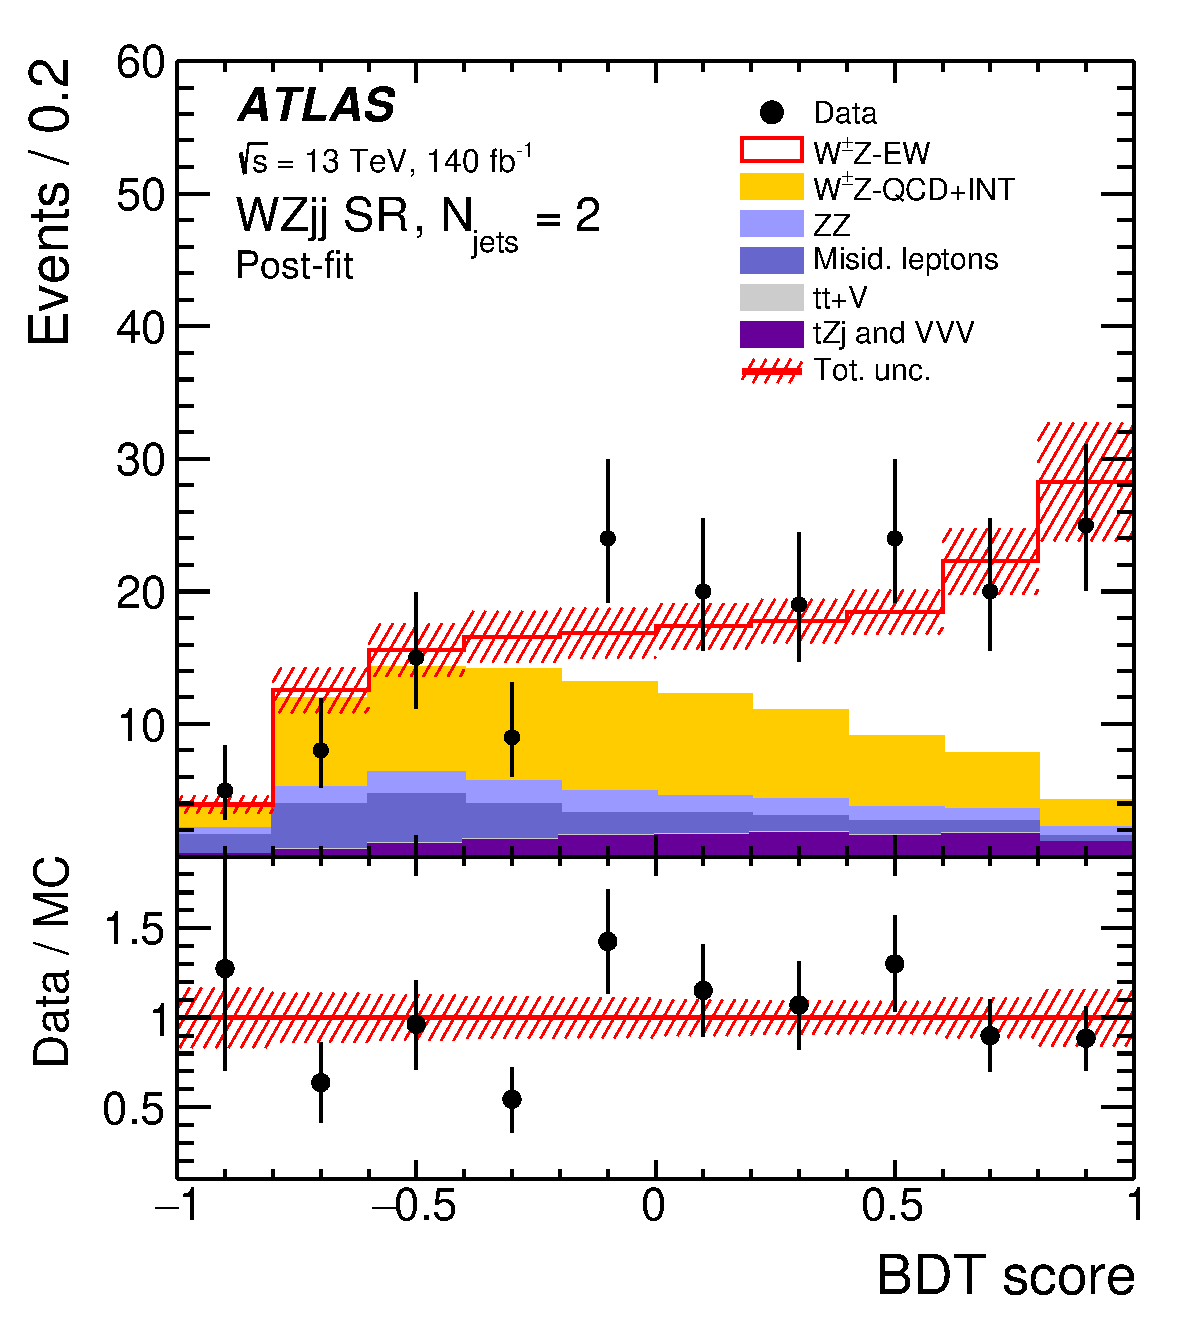
\includegraphics[width=0.39\textwidth]{Immagini/fig_03a.pdf}
        }
        \subfloat[]{
            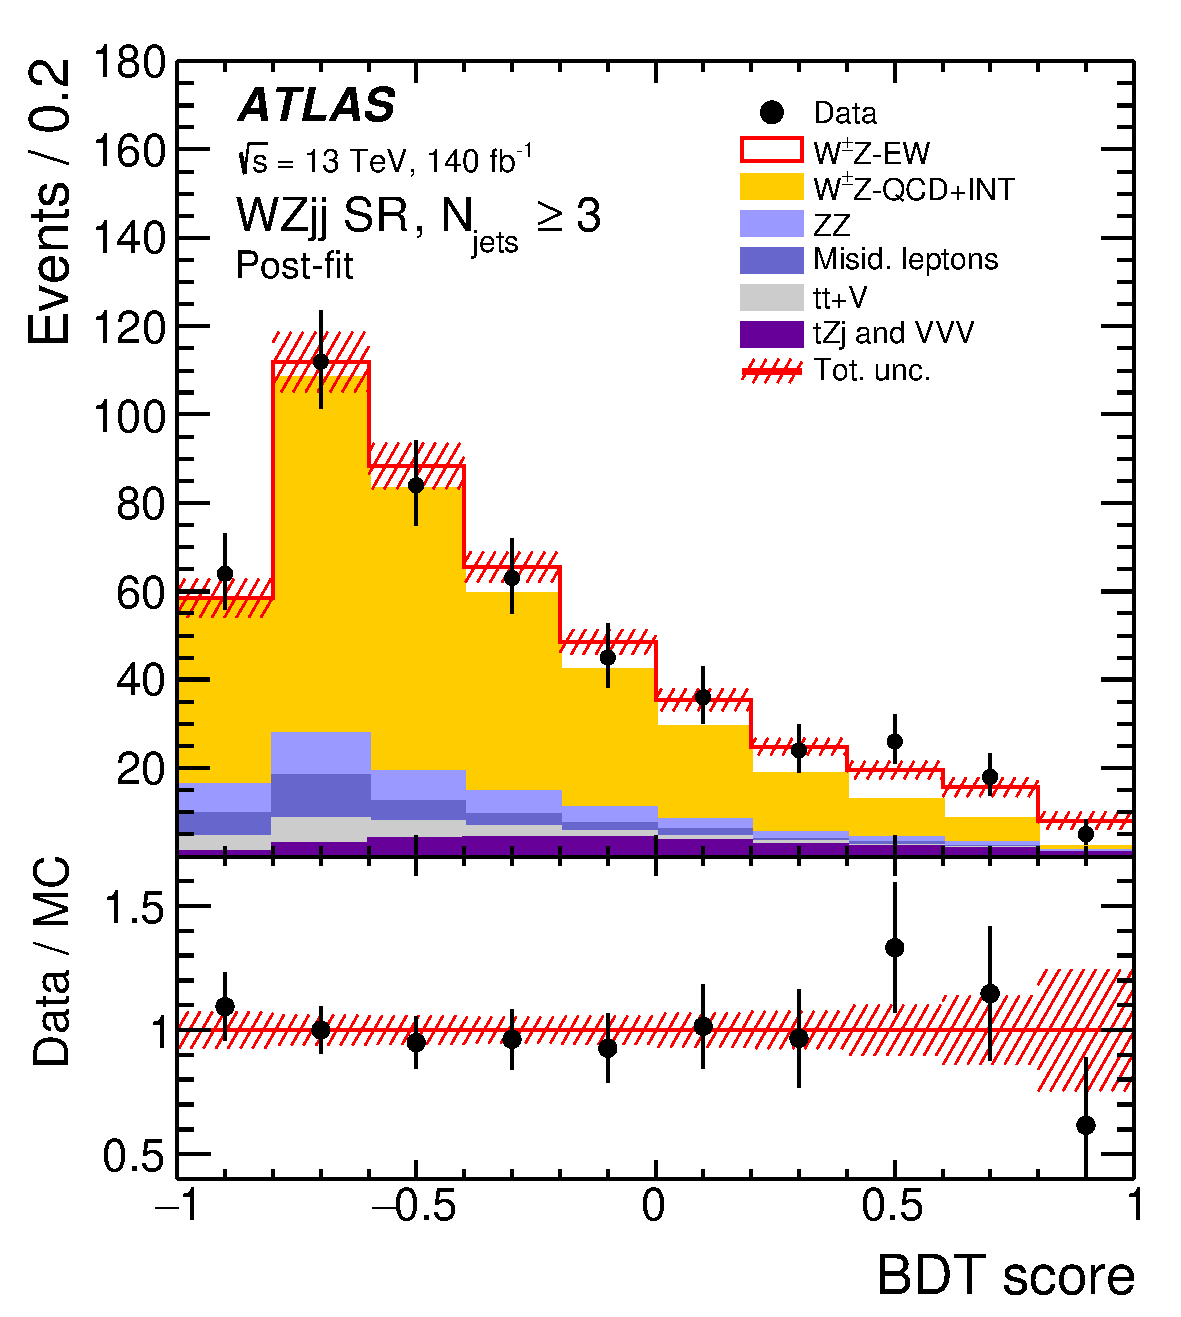
\includegraphics[width=0.39\textwidth]{Immagini/fig_03b.pdf}
        }
    \end{figure}
\end{frame}

\begin{frame}{Post-fit distributions ZZ-CR, b-CR }
    \begin{figure}[t]
        \centering
        \subfloat[]{
            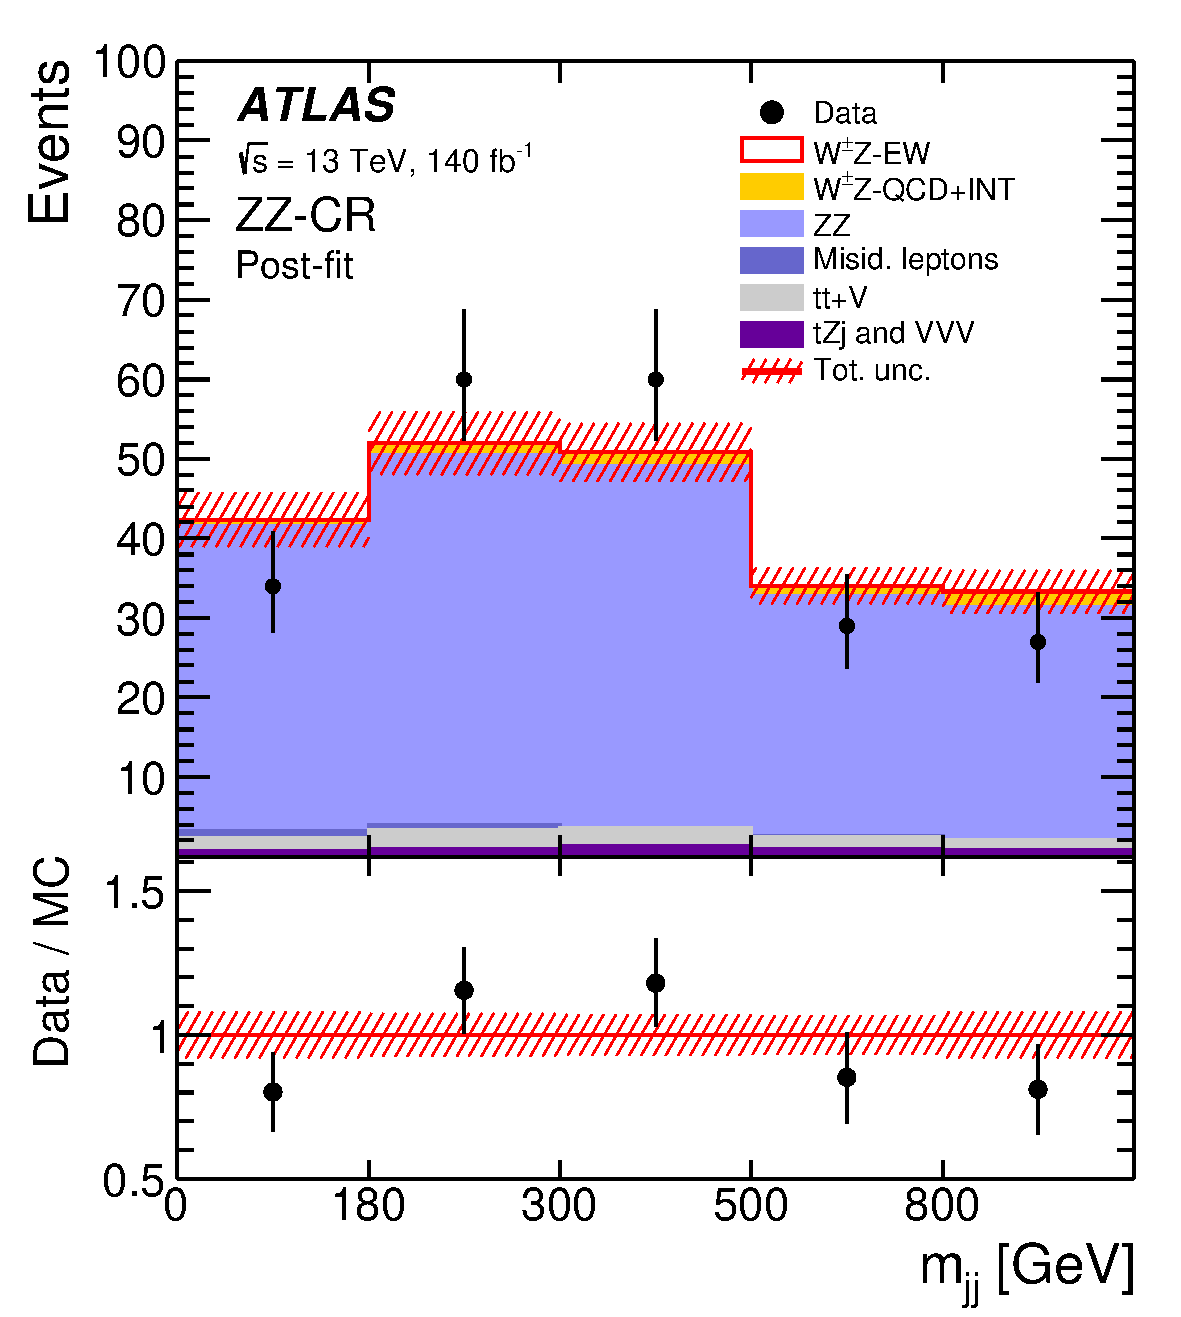
\includegraphics[width=0.39\textwidth]{Immagini/fig_03c.pdf}
        }
        \subfloat[]{
            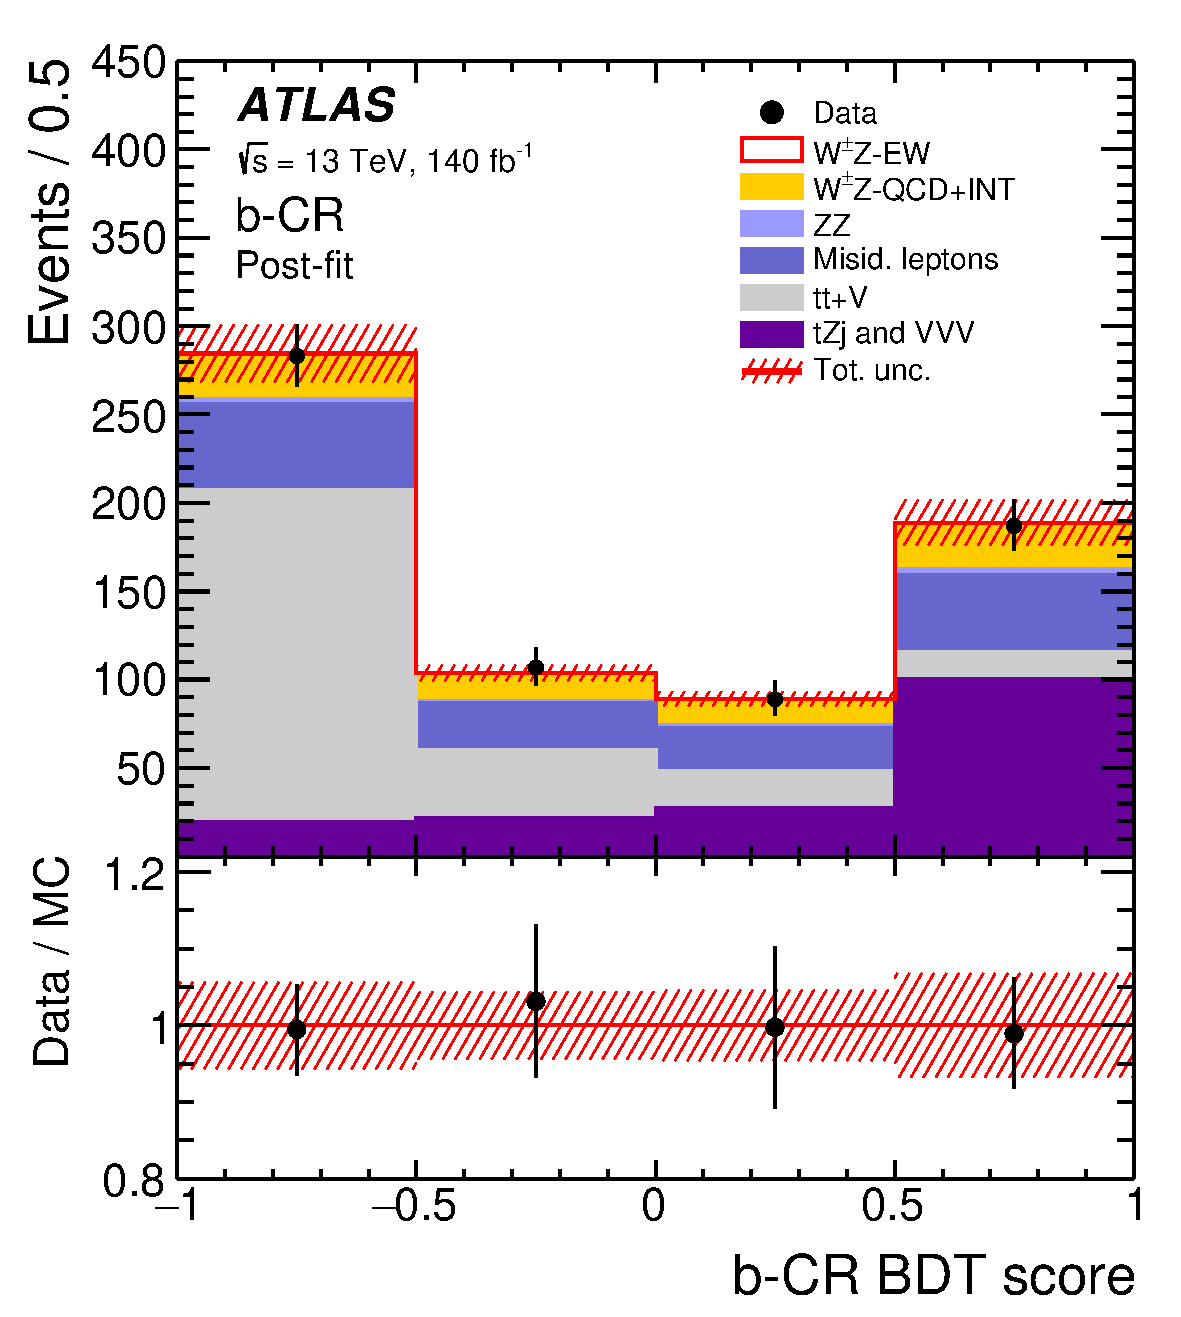
\includegraphics[width=0.39\textwidth]{Immagini/fig_03d.pdf}
        }
    \end{figure}
\end{frame}
\begin{frame}{Fiducial Cross-Section Extraction}    
    The fiducial cross-sections are extracted directly from the profile-likelihood fit. The normalisation factors ($\mu_{EW}$, $\mu_{QCD}$) scale the theoretical MC predictions within the fiducial phase space:
    
    \begin{equation*}
        \sigma_{WZjj-\text{EW}} = \sum_{i} \mu_i^{WZjj-\text{EW}} \cdot \sigma_{i,th.MC}^{WZjj-\text{EW}}
    \end{equation*}
    
    \begin{equation*}
        \sigma_{WZjj-\text{strong}} = \sum_{i} \left( \mu_i^{WZjj-\text{QCD}} \cdot \sigma_{i,th.MC}^{WZjj-\text{QCD}} + \mu_i^{WZjj-\text{INT}} \cdot \sigma_{i,th.MC}^{WZjj-\text{INT}} \right)
    \end{equation*}
    \vspace{0.2cm}
    
    \textit{\scriptsize *Index $i$ runs over the two SR categories: $N_{\text{jets}} = 2$ and $N_{\text{jets}} \geq 3$.}
    
    \vspace{0.3cm}
    \begin{itemize}
        \item \textbf{Interference term:} $\mu_{INT}$ is constrained as $\sqrt{\mu_{EW}} \cdot \sqrt{\mu_{QCD}}$.
        \item \textbf{Categorization:} Splitting by $N_{\text{jets}}$ minimizes the dependency on the MC modelling of QCD radiation.
    \end{itemize}
\end{frame}
\begin{frame}{Results and Comparison with SM Predictions}
    \begin{columns}[T] 
        
        % Colonna Sinistra: I Numeri (leggermente allargata al 52% per far respirare le formule)
        \begin{column}{0.52\textwidth}
            
            % Riquadro Rosso per EWK
            \begin{tcolorbox}[colframe=red!70!black, colback=red!5, boxrule=1pt, arc=4pt, 
                              left=2pt, right=2pt, top=4pt, bottom=4pt, % Riduco i margini interni
                              title=\textbf{VBS (EWK Production)}]
                \centering \small % Centro il testo e lo rimpicciolisco leggermente
                $\sigma_{\text{obs}}^{\text{EWK}} = 0.368 \pm 0.037_{\text{stat}} \pm 0.059_{\text{syst}}\,\unit{fb}$ \\[0.15cm]
                $\sigma_{\text{th}}^{\text{EWK}} = 0.370 \pm 0.030\,\unit{fb}$ \\[0.15cm]
                \textcolor{green!70!black}{$\Rightarrow$ Excellent SM agreement}
            \end{tcolorbox}
            
            \vspace{0.1cm} % Spazio minimo tra i due riquadri
            
            % Riquadro Blu per QCD
            \begin{tcolorbox}[colframe=blue!70!black, colback=blue!5, boxrule=1pt, arc=4pt, 
                              left=2pt, right=2pt, top=4pt, bottom=4pt, 
                              title=\textbf{QCD + Int. (Strong Production)}]
                \centering \small
                $\sigma_{\text{obs}}^{\text{QCD}} = 1.093 \pm 0.066_{\text{stat}} \pm 0.131_{\text{syst}}\,\unit{fb}$ \\[0.15cm]
                $\sigma_{\text{th}}^{\text{QCD}} = 1.537 \pm 0.150\,\unit{fb}$ \\[0.15cm]
                \textcolor{orange}{$\Rightarrow$ Deficit factor $\sim 0.7$ ($1.8\sigma$ tension)}
            \end{tcolorbox}
        \end{column}
        
        % Colonna Destra: Figura 4 del paper
        \begin{column}{0.48\textwidth}
            \begin{center}
                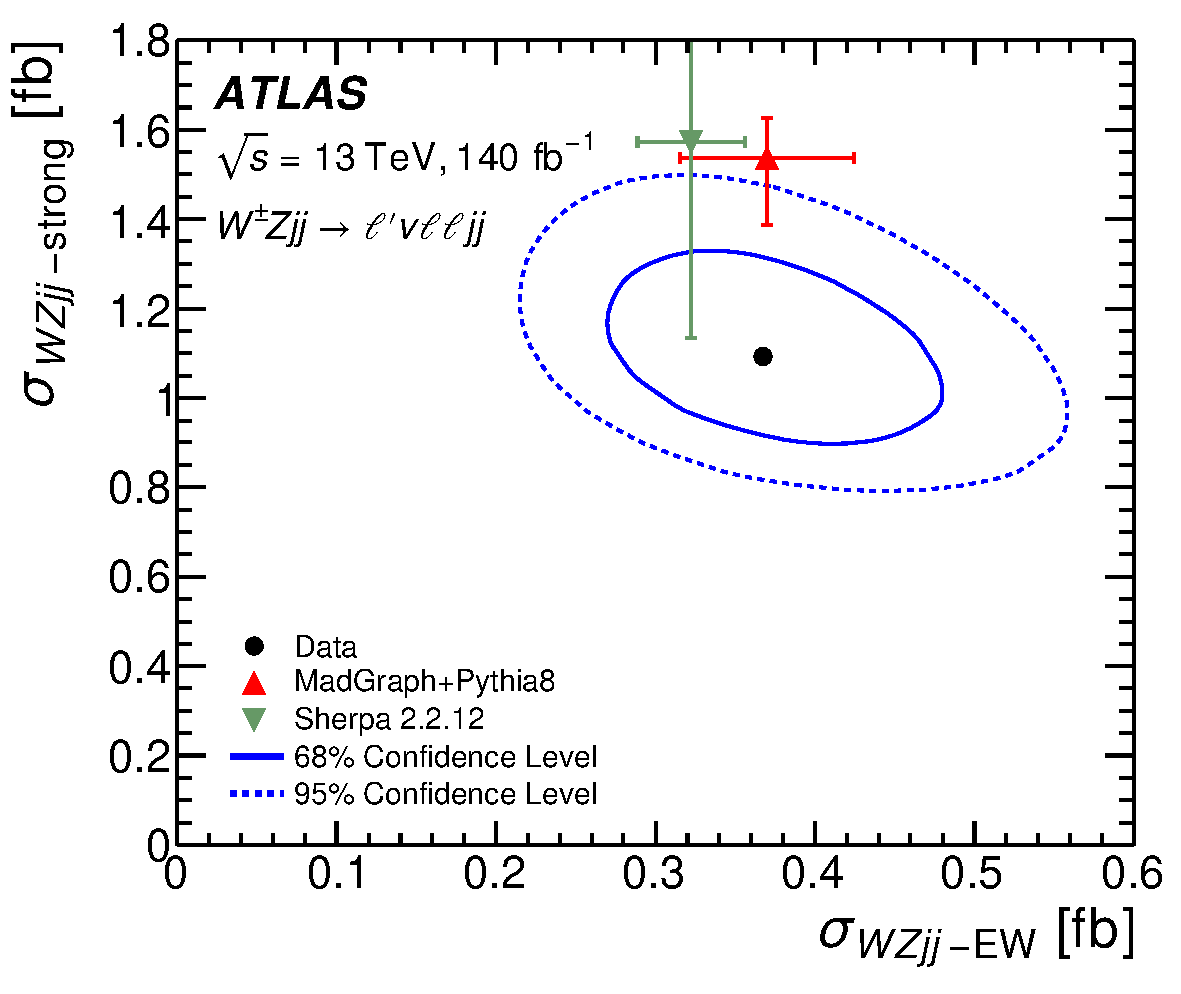
\includegraphics[width=\textwidth]{Immagini/fig_04.pdf}
            \end{center}
        \end{column}
        
    \end{columns}
\end{frame}
\section{Conclusion}